\chapter{Aktueller Stand der Forschung und Praxis}

\section{Ressourcenverbrauch bei KI-Modellen}
\subsection{Ressourcenverbrauch bei KI-Modellen}

substantial challenges in high consumption of computational, memory, energy, and financial resources, especially in environments with limited resource capabilities\footcite[Vgl.][1-2]{baiEfficiencySystematicSurvey2024}

\subsubsection{Nachhaltigkeit}
\subsubsection{Stromverbrauch}
\subsubsection{Rechenleistung begrenzt, KI-Modelle wachsen schneller als verfügbare Leistung}

\section{Neural Networks - Boltzmann Machines}

In recent years, artificial neural networks have first revolutionised computer vision but also other fields, such as natural
language processing, controling and planning (playing games: e.g., Atari and Go), and navigational tasks (finding the shortest path on a map).\footcite[Vgl.][305]{cichyDeepNeuralNetworks2019}
Nowadays, neural networks have reached nearly every feld of science and are a crucial part of various real world applications.\footcite[Vgl.][1513]{gawlikowskiSurveyUncertaintyDeep2023}
Particularly in the last two years, artificial intelligence has also garnered widespread interest from the public, especially regarding chatbots like ChatGPT and Google Bard.\footcite[Vgl.][1-2]{singhChatGPTGoogle2023}  
The most impoortant feature of a neural network-based system that are inspired by our brain, is that they can learn and adapt to data.\footcite[Vgl.][305]{cichyDeepNeuralNetworks2019}

Internally, neural networks are computational models that consist of many simple processing units, called neurons that work together in parallel within interconnected layers.\footcite[Vgl.][305]{cichyDeepNeuralNetworks2019}
They consist out of a network architecture, which describes the layout and how the neurons are wired. Secondly, they have a optimization function which specifies the goals persued in the learning process.\footcite[Vgl.][1583]{durstewitzDeepNeuralNetworks2019}
Lastly, there is a training algorithm that varies all of the hyperparameters, like connection strengths between neurons, training iterations, the learning rate, etc..\footcite[Vgl.][1583]{durstewitzDeepNeuralNetworks2019}
When these interconnected layers are stacked on top of each other the network is called deep.\footcite[Vgl.][305]{cichyDeepNeuralNetworks2019}
Currently, \ac{DNN}s can have up to 1200 interconnected layers that equal to more than 16 million neurons inside the network.\footcite[Vgl.][2]{mallComprehensiveReviewDeep2023}
In genreal, deep learning methods can be seen as subset of machine learning methods and are today's fundament of artificial intelligence.\footcite[Vgl.][1583]{durstewitzDeepNeuralNetworks2019}
For example some regression tasks within computer vision in \ac{DNN} include object detection, medical image registration, head- and body-pose estimation, age estimation and visual tracking.\footcite[Vgl.][325-326]{gustafssonEnergyBasedModelsDeep2020}
Such models can make use of the availability of the recent results in the field of neural networks and deep learning, leading to highly performing, yet very large neural networks with millions of parameters.\footcite[Vgl.][152]{marinoDeepNeuralNetworks2023}
As a result, such models often have a negative effect on the environment in terms of unnecessary energy consumption and a limitation to their deployment on low-resource devices because they are excessively oversized and redundant.\footcite[Vgl.][152]{marinoDeepNeuralNetworks2023}


\subsection{Energy-based models}

An \ac{EBM} is a type of statistical model where the likelihood of a particular state is determined by an energy function.\footcite[Vgl.][2]{huembeliPhysicsEnergybasedModels2022}
Since 1982, those statistical neural network models have been continuously emerging in the machine learning field when J.J. Hopfield introduced the Hopfield Network.\footcite[Vgl.][]{hopfieldNeuralNetworksPhysical1982}
Current developments include their use in reinforcement learning, potential replacements for discriminators in generative adversarial networks and for quantum \ac{EBM}s.\footnote{Vgl.\cite{verdonQuantumHamiltonianBasedModels2019}, p. 1; Vgl.\cite{duModelBasedPlanning2021}, p. 1}
In addition to that, Open AI showed that \ac{EBM}s are useful models across a wide variety of tasks like achieving state-of-the-art out-of-distribution classification and continual online class learning to name a few.\footcite[Vgl.][1-2]{duImplicitGenerationGeneralization2020}
The underlying idea behind \ac{EBM}s is to establish a probabilistic physical system that is able to learn and memorize patterns but most importantly generalize it.\footcite[Vgl.][2]{huembeliPhysicsEnergybasedModels2022} 
Especially, it involes learning an energy function \(E_{\theta}(x) \in \mathbb{R}\) and assigning the low energy to observed data \(x_i\) and high energy to other values \(x\).\footcite[Vgl.][330]{gustafssonEnergyBasedModelsDeep2020}
\begin{figure}[H]
    \centering
    \fbox{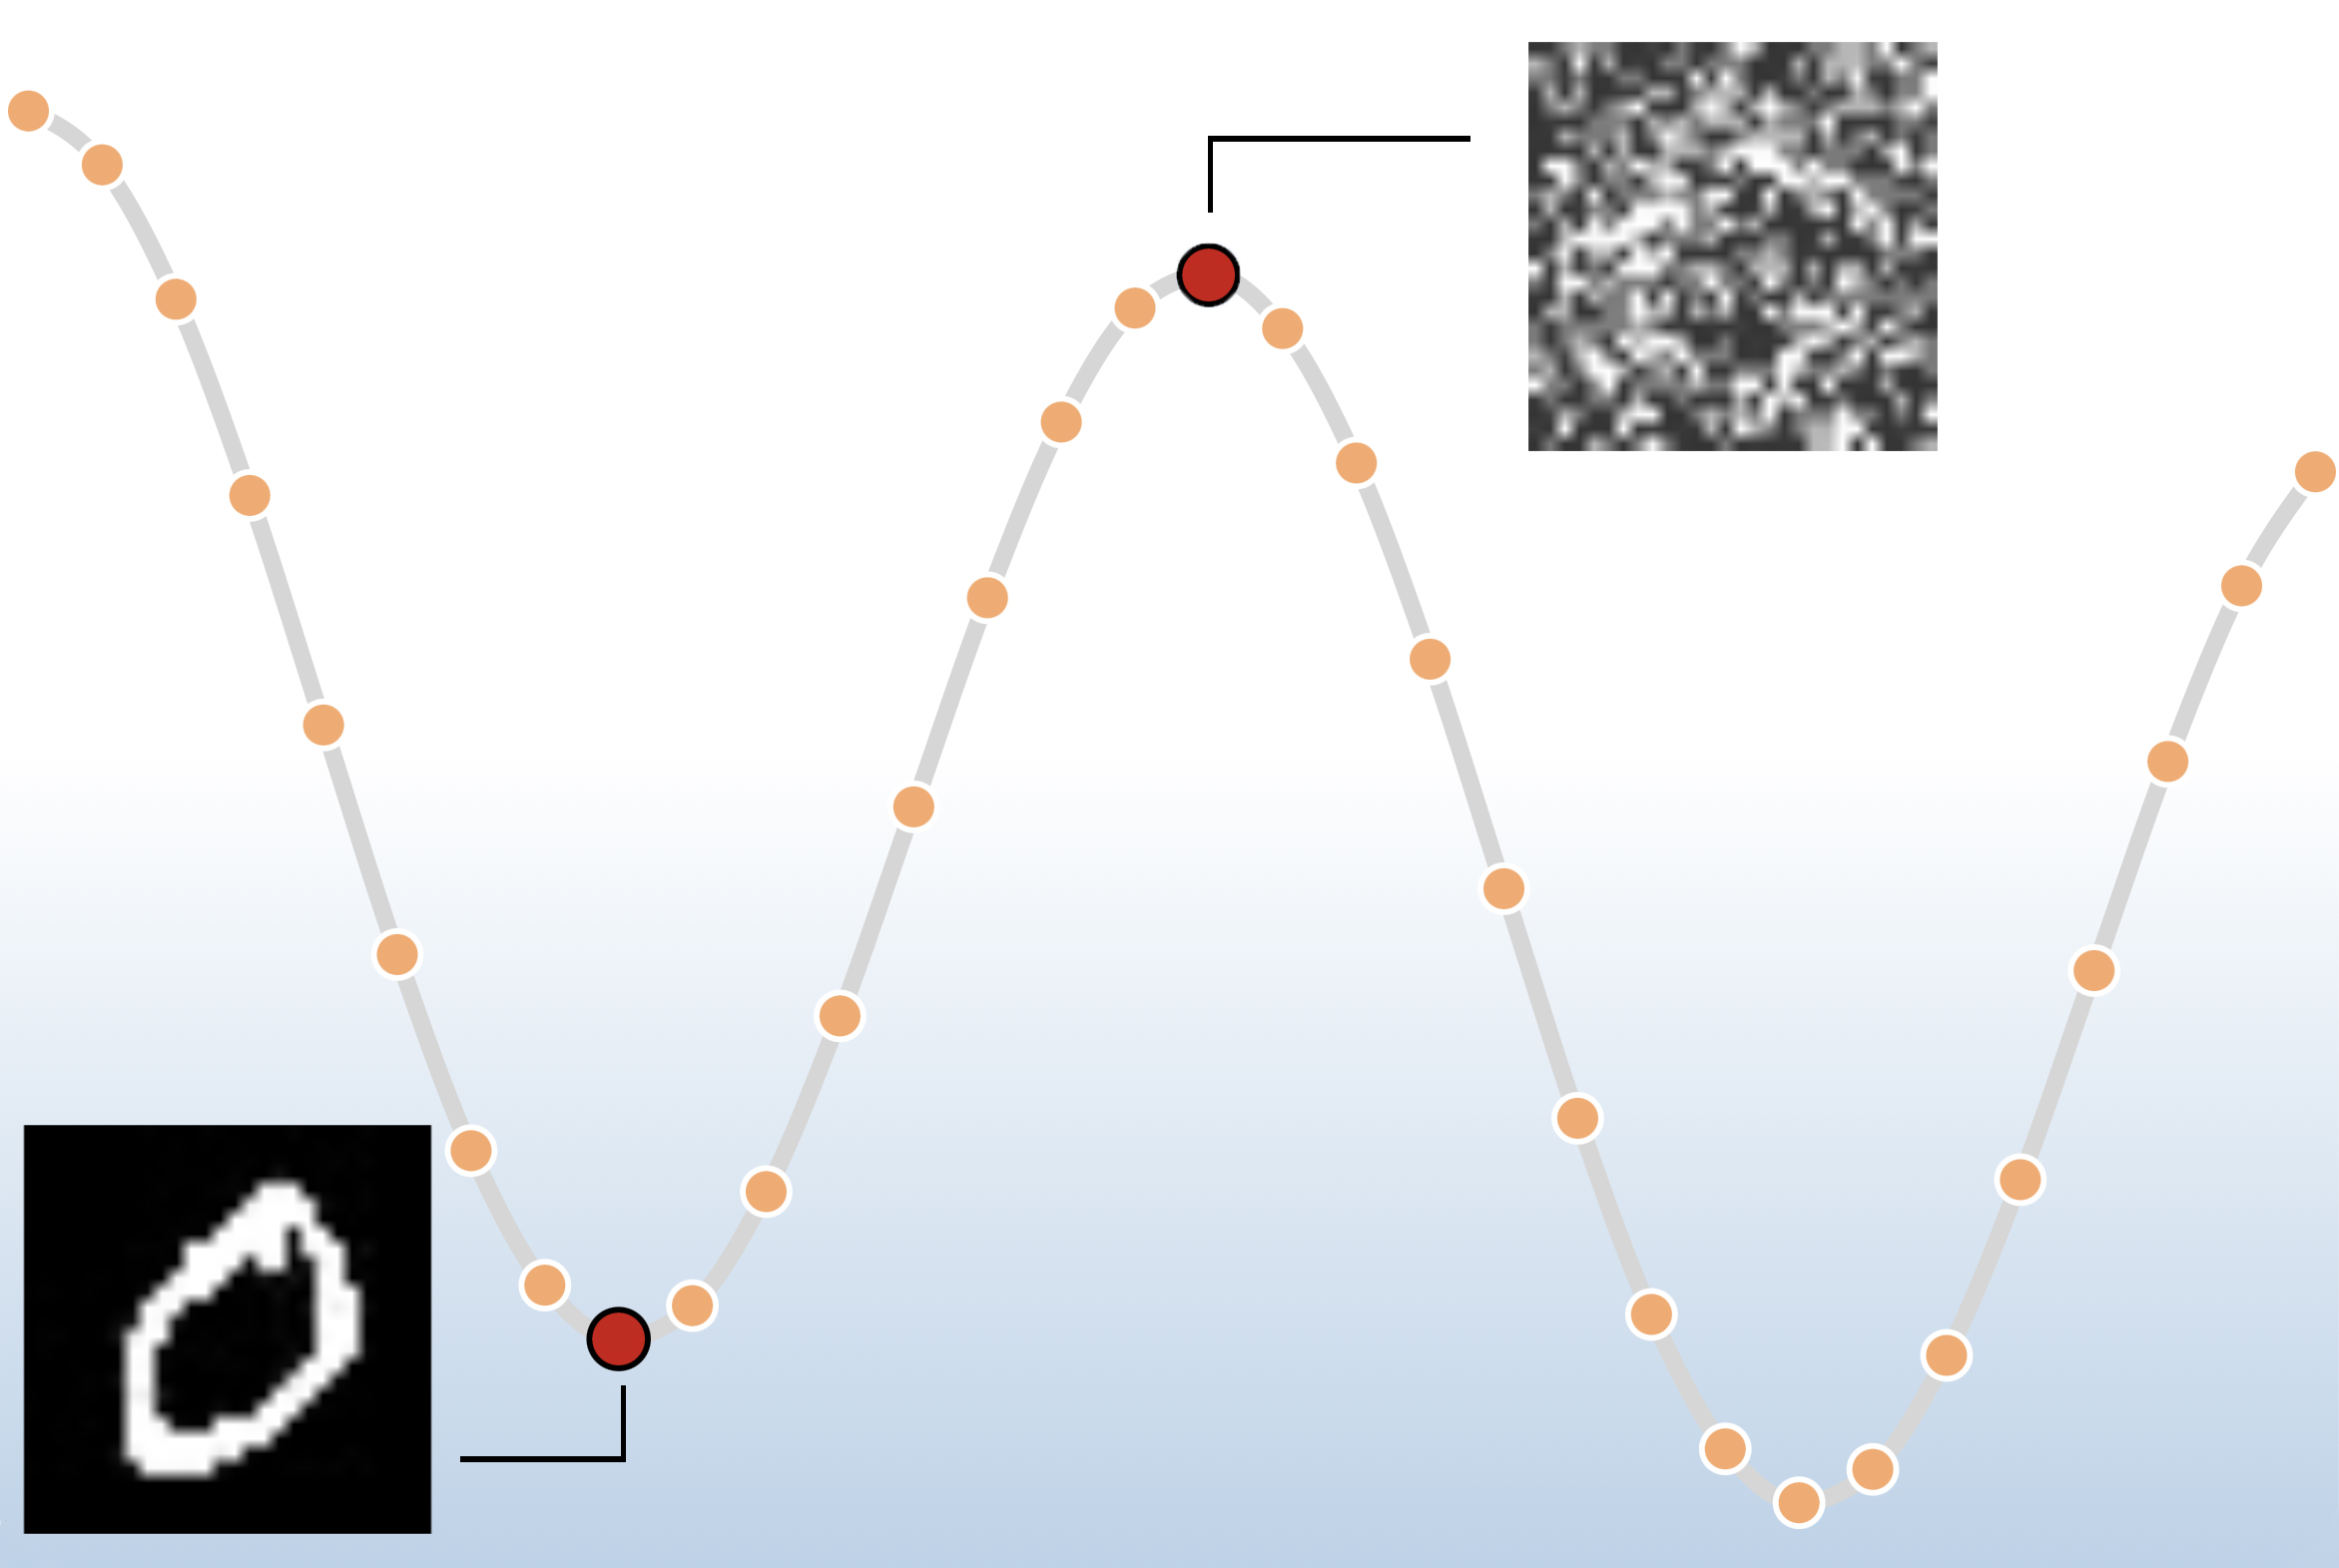
\includegraphics[width=0.4\linewidth]{graphics/energielandschaft.jpg}}
    \caption{Figure of a simplified energy landscape}
\end{figure}
In this figure 1 a simplified energy landscape is shown where the local minima correspond to states that encode an MNIST digit.\footcite[Vgl.][6]{huembeliPhysicsEnergybasedModels2022} It is visible that observed data settles in the local minimum of the energy landscape, in this case a clear 0. On the other hand close to the local maxima of the energy landscape the 0 is only barely recognizable and therefore got a higher energy value assigned to it.
The assumption of the underlying distribution function \( P(x) \)  is equal to the solution of the optimization problem:
\begin{equation}
    P(x) = \frac{1}{Z} \exp\left(-\frac{E(x)}{T}\right),
\end{equation}
where \( Z \) is given by the partition function to ensure
that the density function normalizes to a total probability of 1 and \( T \) is interpreted as the temperature .\footcite[Vgl.][2-3]{huembeliPhysicsEnergybasedModels2022}
As a result the behavior of a \ac{EBM} is determined by 2.1. 
The aim of the training is to match the real data \( P_{\text{data}} \) as closely as possible with the internal model \( P_{\text{model}} \).
A practical method to achieve this goal is to use the KL divergence. KL divergence is a mathematical equation that helps to meassure how close the predictions are by comparing the model's learned distribution to the true distribution of the data:
\begin{equation}
    G = \sum_x P^+(x) \ln \left( \frac{P^+(x)}{P^-(x)} \right)
\end{equation}
Here, \(P^+(x)\) is the probability when the states are determined by a data input from the environmnet, while \(P^-(x)\) represents the internal network running freely, also referred to as ``dreaming''.\footcite[Vgl.][154-155]{ackleyLearningAlgorithmBoltzmann1985}
To optimise the KL divergence, in this case \( G \), the energy is adjusted, whereby data is assigned to low energy states (according to 2.1) and the training data receives high energy and therefore high probabiliies.\footcite[Vgl.][2-3]{zhaiDeepStructuredEnergy2016}
To complete the section the ``partition function'', \( Z \), used in 2.1 is given by summing over all possible pairs of visible and hidden vectors:
\begin{equation}
    Z = \sum_x \exp\left(-\frac{E(x)}{T}\right)
\end{equation}
As a side note it is worth mentioning that using the maximum likelihood estimator for \( Z \) is intractable due to the requirement of summing over all possible states, which leads to an exponential increase in the number of states for larger systems.\footcite[Vgl.][2-3]{zhaiDeepStructuredEnergy2016}

\subsection{concept of Boltzmann Maschines}

A \ac{BM} is a specific symmetrical \ac{EBM} consisting of binary neurons \{0, 1\}.\footcite[Vgl.][260]{amariInformationGeometryBoltzmann1992}
The neurons of the network can be split into two functional groups, a set of visible neurons and a set of hidden neurons.\footcite[Vgl.][154]{ackleyLearningAlgorithmBoltzmann1985}
Therefore, the \ac{BM} is a two-layer model with a visible layer (``v'') and a hidden layer (``h'').\footcite[Vgl.][448]{salakhutdinovDeepBoltzmannMachines2009}
The visible layer is the interface between the network and the environment. It receives data inputs during training and sets the state of a neuron to either \{0, 1\} which represents activated or not activated.
On the other hand, the hidden units are not connected to the environment and can be used to “explain” underlying constraints in the internal model of input vectors and they cannot be represented by pairwise constraints.\footcite[Vgl.][154]{ackleyLearningAlgorithmBoltzmann1985}
The connection between the individual neurons is referred to as bidirectional, as each neuron communicates with each other in both directions.\footcite[Vgl.][149]{ackleyLearningAlgorithmBoltzmann1985}

As early as 1985, one of the founding fathers of artificial intelligence, ``Geoffrey Hinton'', was aware that an \ac{BM} is able to learn its underlying features by looking at data from a domain and developing a generative internal model.\footcite[Vgl.][148]{ackleyLearningAlgorithmBoltzmann1985}
In the next step, it is possible to generate examples with the same probability distribution as the input data examples shown.
In the following figure \ref{fig1}, a general \ac{BM} is depicted, where the upper layer embodies a vector of stochastic binary 'hidden' features, while the lower layer embodies a vector of stochastic binary 'visible' variables.\footcite[Vgl.][449]{salakhutdinovDeepBoltzmannMachines2009}

\begin{figure}[H]
    \centering
    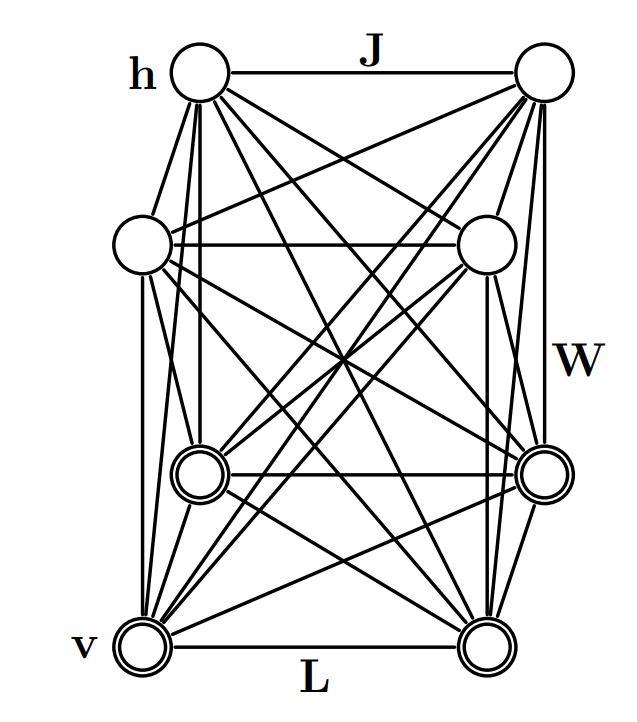
\includegraphics[width=0.25\linewidth]{graphics/General_BM.png}
    \caption{figure of a general Boltzmann Machine}
    \label{fig1}
\end{figure}
The model contains a set of visible units \( v \in \{0, 1\} \), and a set of hidden units \( h \in \{0, 1\} \) (see Fig. 1). The energy function of the \ac{BM} with the states \( \{v, h\} \) is defined as:
\begin{equation}
E(v, h; \theta) = -\frac{1}{2} v^T L v - \frac{1}{2} h^T J h - v^T W h,
\end{equation}

where \( \theta = \{W, L, J\} \) are the model parameters.\footcite[Vgl.][448]{salakhutdinovDeepBoltzmannMachines2009}
\( W, L, J \) represent visible-to-hidden, visible-to-visible and hidden-to-hidden weights.
The individual neurons can be made to try to minimize the global energy by setting the right assumptions.\footcite[Vgl.][150]{ackleyLearningAlgorithmBoltzmann1985}
Entering a particular input to the machine, the system will find the minimum energy configuration that can illustrate the input.\footcite[Vgl.][150]{ackleyLearningAlgorithmBoltzmann1985}
A simple method to find a local energy minimum is to switch into wichever of the two states of a neuron hold the lower energy given the current state of the other neurons.\footcite[Vgl.][110]{fahlmanMassivelyParallelArchitectures1983}  
The exact reason for this is the following: ``If all the connection strengths are
symmetrical, which is typically the case for constraint satisfaction
problems, each unit can compute its effect on the total energy from
information that is locally available.''\footcite[110]{fahlmanMassivelyParallelArchitectures1983}  
By inserting the function 2.4 into the earlier introduced KL-divergence 2.2 and doing gradient descend the following learning rule to update the weights and biases results\footcite[Vgl.][5]{hintonPracticalGuideTraining2012}:

\begin{equation}
    \Delta w_{ij} = \epsilon ( \langle v_i h_j \rangle_{\text{data}} - \langle v_i h_j \rangle_{\text{model}} )
\end{equation}

The network can now update the weights ``W'' that exist between the neurons through the training rule based on the observations that served as input and modified by the learning rate \(\epsilon\).\footcite[Vgl.][1-2]{barraEquivalenceHopfieldNetworks2012}

Performing exact maximum likelihood learning in this model is intractable because exact computation of the data predictions and the model predictions takes a time that is exponential in the number of hidden units.\footcite[Vgl.][449]{salakhutdinovDeepBoltzmannMachines2009}
When the number of hidden units is large compared to the number of visible units it is impossible to achieve a perfect model because of the totally connected network and the resulting \( 2^n \) possbilities.\footcite[Vgl.][154]{ackleyLearningAlgorithmBoltzmann1985}
This leads back to the briefly mentioned constraint of equation 2.3, that is needed to calculate an activation probability of a neuron, which is required to update a weight in the training process shown in 2.5.

A specific example to demonstrate why it is intractable to calculate a activiation of a \ac{BM} is the following. A fictional \ac{BM} has 80 visible nodes and 120 hidden nodes and therefore the possbilities of states of neurons are \( 2^{200} \), which is \( 1.61 \times 10^{60}\). 
To put this in perspective the toal atoms that exist on earth are only estimated to be around \( 1.33 \times 10^{50}\).\footnote{Vgl.\cite{helmenstineHowManyAtoms2022}, p. 478-480; Vgl.\cite{schlammingerCoolWayMeasure2014}, p. 1}
That means even if it would be possible to store one information per atom it would just not be enough. 

\subsection{Training of Restriced Boltzmann Machines}

As a solution for the training problem Hinton and Sejnowski proposed Gibbs sampling as an algorithm to aporoximate both expectations.\footcite[Vgl.][158-165]{ackleyLearningAlgorithmBoltzmann1985}
Furthermore, the intralayer connections of the model got removed and the result is the so called \ac{RBM}.
To transform an \ac{BM} into a \ac{RBM} the diagonal elements \( L \) and \( J \)  introduced earlier, are set to 0 and as a result the well-known model of a \ac{RBM} establishes shown in fig.2.\footcite[Vgl.][449]{salakhutdinovDeepBoltzmannMachines2009}

\begin{figure}[H]
    \centering
    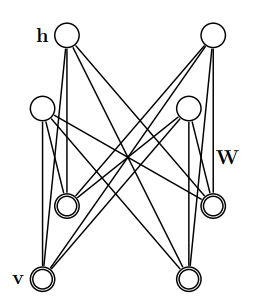
\includegraphics[width=0.25\linewidth]{graphics/RBM_Modell.png}
    \caption{Figure of a \ac{RBM}}
\end{figure}
What can be recognized that no more visible-to-visible and hidden-to-hidden connections can be found in the model.
The configuration of the visible and hidden units \( (v, h) \) therefore has also an updated energy function (Hopfield, 1982) given by:
\begin{equation}
E(v, h) = - \sum_{i \in \text{visible}} a_i v_i - \sum_{j \in \text{hidden}} b_j h_j - \sum_{i,j} v_i h_j w_{ij},
\end{equation}
where \( v_i, h_j \) are the binary states of a visible unit \( i \) and hidden unit \( j \), \( a_i, b_j \) are their biases and \( w_{ij} \) is the weight between them.\footcite[Vgl.][3-4]{hintonPracticalGuideTraining2012a}
Despite, compared to the fully connected \ac{BM}, the \ac{RBM} is less complex but the advantages of training surpasses the loss in expressivity.\footcite[Vgl.][4]{huembeliPhysicsEnergybasedModels2022}
The \ac{RBM} has recently been drawing attention in the machine learning community beceause of its adaption and extention for various tasks such as representational learning, document modeling, image recognition and for
serving as foundational components for deep networks including Deep Boltzmann Machines, Deep Belief Networks and hybrid models with CNNs.\footcite[Vgl.][1186]{zhangOverviewRestrictedBoltzmann2018}
The training of the model can be split up into the following steps:

\textbf{1. Forward Pass (positive phase)}

During the forward pass using the Gibbs Sampling method, the visible units are set to a completely random state. Next up the hidden units are computed.
The computation of the hidden units involves calculating their acitivation probabilities and performing an actual sampling with their calculated activation probabilities.
With the \ac{RBM} it is now easy to get an analytical calculated unbiased sample of $(\textbf{v}_i\textbf{h}_j)_{data}$.\footcite[Vgl.][5]{hintonPracticalGuideTraining2012}
Given an input data out of the training images, \( v \), the binary state, \( j \), of each hidden unit,  \( h_j \), is set to 1 with following probability:

\begin{equation}
p(h_j = 1 | \textbf{v}) = \sigma(b_j + \sum_i v_i w_{ij}),
\end{equation}
where $\sigma(x)$ is the logistic sigmoid function with an unbiased sample. The sigmoid function is defined as $\sigma(x) = \frac{1}{1 + \exp(-x)}$ and shown in figure 4:
\begin{figure}[H]
    \centering
    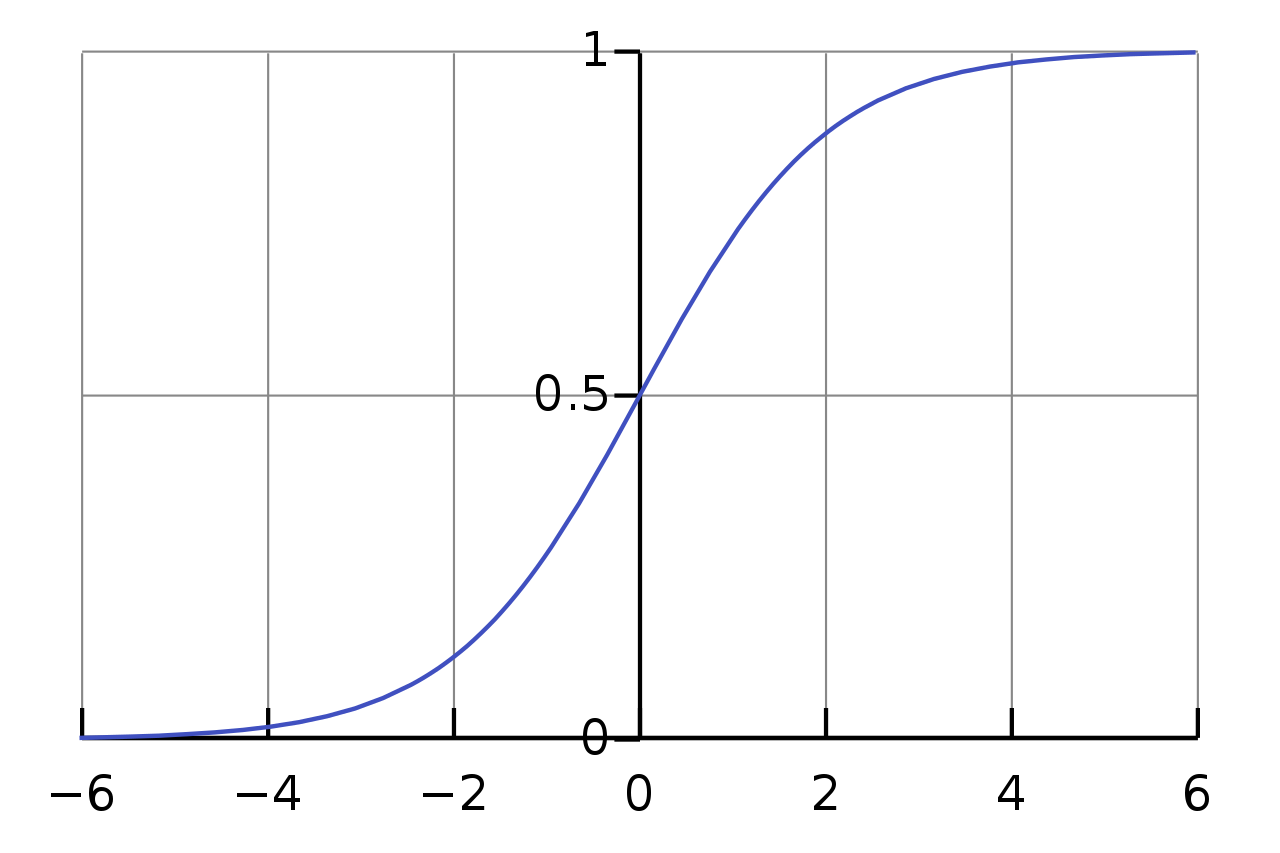
\includegraphics[width=0.5\linewidth]{graphics/logistic_sigmoid.png}
    \caption{Figure of a logistic sigmoid function \ac{RBM}}
\end{figure}
The result is a set of probabilities that reflect how likely it is for each hidden unit to be on or off given the input data.\footcite[Vgl.][6]{huembeliPhysicsEnergybasedModels2022}
The sampling part of the positive phase uses the just calculated acitivation probabiliy of each hidden unit and performs a random experiment with it.
Afterwards, the hidden unit is either activated or not activated and the training process continues with the new state of the hidden units (activated or not activated).

\textbf{2. Reconstruction (negative phase)}

In this phase, the sampled hidden states are used to reconstruct the visible units. 
This is essentially a prediction of the input, which is calulated with following probability:\footcite[Vgl.][6]{hintonPracticalGuideTraining2012}
\begin{equation}
    p(v_i = 1 | \mathbf{h}) = \sigma(a_i + \sum_j h_j w_{ij})
\end{equation}
The sampling part of the negative phase uses the just calculated acitivation probabiliy
of each visible unit and performs a random experiment, like in the positive phase.
Now, the result is a prediction of the input in the visible nodes.
Afterwards, a half forward pass is made to calculate the activation probability of a hidden unit again based on the activated or not activated visible units.

\textbf{3. Updating the weights}

Meanwhile, all the requirements to update the weights are satisfied and can be used within the equation 2.5. 
The delta that results is summed to the current weight and therefore the internal model gets closer to prediciting the observed data.
Therefore, one training iteration consisting out of 1 Forward Pass, 1 Reconstruction and 0.5 Forward Pass again is accomplished.
Repeating this training steps \( N \) times for a suitable chosen \( N \) the model learns better, since more steps of alternating Gibbs sampling were performed.\footcite[Vgl.][6]{huembeliPhysicsEnergybasedModels2022}


\subsubsection{Markov-Chain-Monte-Carlo-Verfahren}

\textbf{Contrastive Divergence:} Contrastive divergence is a special Gibbs Sampling training method
developed by Geoffrey Hinton for the efficient training of Boltzmann Machines, especially \ac{RBM}s.\footcite[Vgl.][4-5]{hintonPracticalGuideTraining2012}
In traditional Gibbs sampling would have to generate a long chain of samples, until
independent samples are obtained from the observed data distribution of the model.\footcite[Vgl.][5-6]{huembeliPhysicsEnergybasedModels2022}
The samples are needed for each iteration of the gradient ascent on the log-likelihood
resulting in large computational costs.\footcite[Vgl.][7-8]{upadhyaOverviewRestrictedBoltzmann2019}
To solve this issue contrastive divergence minimizes an approximation of the Kullback-Leibler divergence between the empirical distribution of the training data and the distribution generated by the model.\footcite[Vgl.][246]{mocanuTopologicalInsightRestricted2016}
They way to achieve this is by initializing the Markov chain with the samples from the data distributon.\footcite[Vgl.][7-8]{upadhyaOverviewRestrictedBoltzmann2019}
The outcome has been shown to heavily increase the training time while only adding a small bias.\footcite[Vgl.][537]{larochelleClassificationUsingDiscriminative2008}
What this means is initializing the visible units with a real data input for example a MNIST sample and starting the proposed steps with the underlying states.
Often the process can be stopped after only sampling a very small number of steps (often only one).\footcite[Vgl.][646]{larochelleLearningAlgorithmsClassification2012}


\textbf{Metropolis-Hastings:} The Metropolis-Hastings algorithm, often only called Metropolis algorithm, is a technique out of \ac{MCMC} class techniques.\footcite[Vgl.][1]{patronOptimalRelaxationRate2024}
The Metropolis-Hastings method was invented by Metropolis et al. in 1953 when he noticed, that for an intractable distribution with too many states it can be seen as a limiting distribution of Markov chains.\footcite[Vgl.][1087-1092]{metropolisEquationStateCalculations1953}
The goal of the technique is to create a sequence of correlated steps from a random walk that, after enough iterations, makes it possible to sample a desired target probability distribution.\footcite[Vgl.][1]{patronOptimalRelaxationRate2024} 
The intractable distribution to handle with the Metropolis-Hastings technique in the case of \ac{RBM}s is equation 2.3.
An Interpretation of the method can be expressed as: "A visitor to a museum that is forced by a general blackout to watch
a painting with a small torch.
Due to the narrow beam of the torch, the person cannot get a global view of the painting but can proceed along this painting until all parts have been seen."\footcite[Vgl.][2]{robertMetropolisHastingsAlgorithm2016}
The version already adjusted for \ac{RBM}s incorporates the following functionality of the Metropolis technique:

First, select a random or given configuarion $x_{\text{old}}$ of a \ac{RBM} that holds the states of all visible and hidden neurons.\footcite[Vgl.][65]{beichlMetropolisAlgorithm2000}
Secondly, the energy of the configuration, noted as  $E_{\text{old}}$, must be calculated using Equation 2.6, as previously introduced. Subsequently, this energy value is stored.
Thirdly, the configuration gets updated by picking one random neuron and changing the state of it from 0 to 1 or vice versa.\footcite[Vgl.][1]{rosenthalOptimalProposalDistributions2009}
This new configuration is stored as $x_{\text{new}}$. Following that the energy of the new configuration $E_{\text{new}}$ is calculated and stored.
Now the two energy values are compared and if $E_{\text{new}}$ < $E_{\text{old}}$ the new configuration will be accepted and $x_{\text{old}}$ = $x_{\text{new}}$.\footcite[Vgl.][1-2]{patronOptimalRelaxationRate2024}
If $E_{\text{new}}$ > $E_{\text{old}}$ then there are some extra steps to be followed: 

The flip probability is calculated as $p=\exp\left(-\frac{E_{\text{new}}-E_{\text{old}}}{kT}\right)$.
\( KT \) is interpreted as the temperature in the network and with higher temperature it increases
the acitivation probability leading to an faster exploration through the landscape but with less details.\footcite[Vgl.][1-9]{liTemperatureBasedRestricted2016}
For \ac{RBM}s \( KT \) is assumed to be 1. (FOOTCITE von Fabian fehlt). In the following figure 5 the resulting probability function is shown.

\begin{figure}[H]
    \centering
    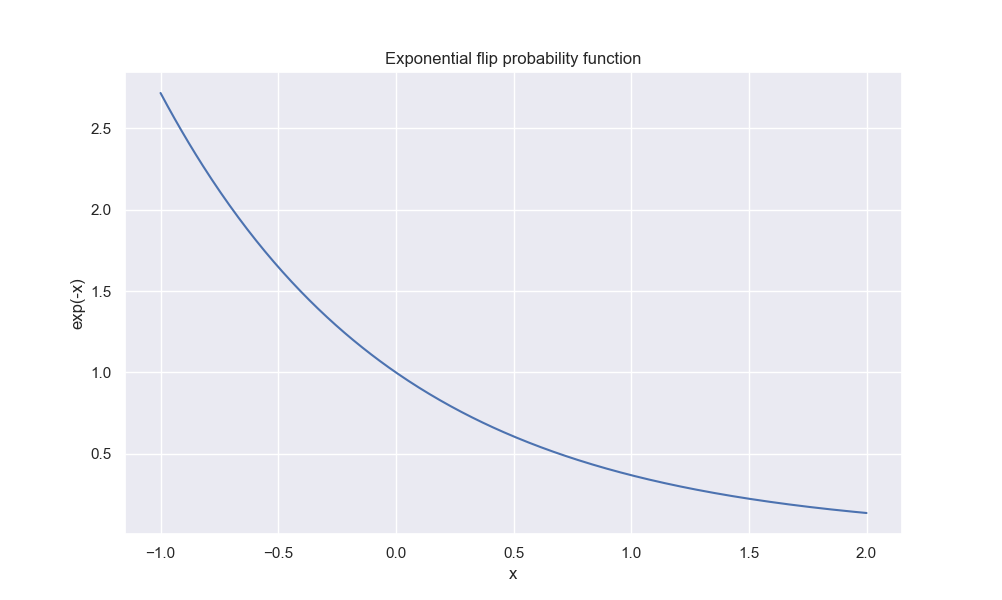
\includegraphics[width=0.7\linewidth]{graphics/Exponential flip probability function.png}
    \caption{Figure of the exponential flip probability function}
\end{figure}

In the next step a uniform random number $r$ between 0 and 1 is generated.
After generating $r$ the configuration will be accepted if $r \leq p$ (i.e., $x_{\text{old}}=x_{\text{new}}$).\footcite[Vgl.][2-3]{patronOptimalRelaxationRate2024}
Otherwise, a rejection takes place if $r > P$ (i.e., $x_{\text{old}}=x_{\text{old}}$).

Finally, the configuration $x_{\text{old}}$ can be stored and the process repeats beginning from step 2 on.\footcite[Vgl.][17]{patronOptimalRelaxationRate2024}
After repeating enough times the activation probability for each neuron can be calculated by summing over all samples $(x_1+x_2+x_3+\ldots)$ and the result is divided by the total number of samples.


\subsection{Current Problems witht BMs and RBMs}

One general problem that occurs in the learning process of a \ac{BM} is that it is both time-consuming and difficult.\footcite[Vgl.][1-2]{fischerIntroductionRestrictedBoltzmann2012}
This is because sampling from an undirected graphical model is not straightforward and therefore \ac{RBM}s can make use
of \ac{MCMC} proposed methods like Contrastive Divergence and Metropolis Hastings.\footcite[Vgl.][2]{fischerIntroductionRestrictedBoltzmann2012}
In addition to that, the selection of hyperparameters can be difficult since for the training of a practical model a large hyper-parameter space needs to be explored.\footcite[Vgl.][536]{larochelleClassificationUsingDiscriminative2008}
Especially finding the right size of the hidden layer, the learning rate and number of training iterations but also the method for calculating activation probabilities(Contrastive Divergence, Metropolis Hastings, etc.) can be seen as art.
Furthermore, training can become unstable due to the system's low temperature, which impacts the training negatively.\footcite[Vgl.][3-4]{huembeliPhysicsEnergybasedModels2022}
A lower temperature reduces the system's possbility to explore the energy landscape thoroughly, leading to the false selection of local minima instead of finding the global minimum.

\section{Hardwarebeschleuniger}
\subsection{Aktuelle Ansätze im Bereich KI und weitere Lösungen}
\subsubsection{Asics}
\subsubsection{Quantencomputing}
\subsection{ISING Maschine/ Physikinspirierter Hardwarebeschleuniger}
\subsubsection{Konzept (mit Energiefunktion), Probleme der Digitalrechner bzw. Unterschied zu Digitalrechner}
\subsubsection{Aktuelle Anwendung}
\subsubsection{Potentielle Einsatzgebiete für KI-Modelle}
\subsubsection{Parallelen Energiefunktion BM und ISING Maschine}

\section{Memristor Hopfield Network}
\subsection{Memristor}
\subsection{Hopfield Network}

A Hopfield Network is an \ac{EBM} and belongs to the field of recurrent neural networks.\footcite[Vgl.][35]{dramschChapterOne702020}
The structure of the network consists of only one single layer with binary valued neurons inside.\footcite[Vgl.][7]{ahadNeuralNetworksWireless2016}
Therefore, the neurons state can either be \{1, 0\} or \{1, -1\}.
The connections between the neurons are symmetrical, which means that the weights of the connections are the same in either direction.\footcite[Vgl.][7]{ahadNeuralNetworksWireless2016}
Initially, the primary applications of this type of network were to serve as storage for associative patterns and to facilitate pattern retrieval.\footcite[Vgl.][2]{ramsauerHopfieldNetworksAll2021}
In practive given a query pattern a Hopfield Network can retrive a pattern that is most similar or an is an average of similar patterns.\footcite[Vgl.][2]{ramsauerHopfieldNetworksAll2021}
In this paper the Hopfield Network's update function interests us because it possibly could be used to sample the intractable training of a \ac{RBM} mentioned earlier.
Surprisingly, since Hopfield networks were introduced by J.J Hopfield in 1982 the storage capacity got increased over time but the fundamentals stayed the same.\footnote{Vgl.\cite{hopfieldNeuralNetworksPhysical1982}, p. 2554-2558; Vgl.\cite{ramsauerHopfieldNetworksAll2021}, p. 2}
In following figure 6 an example of a Hopfield Network can be seen.\footcite[Vgl.][1-2]{yaoMassivelyParallelAssociative2013}

\begin{figure}[H]
    \centering
    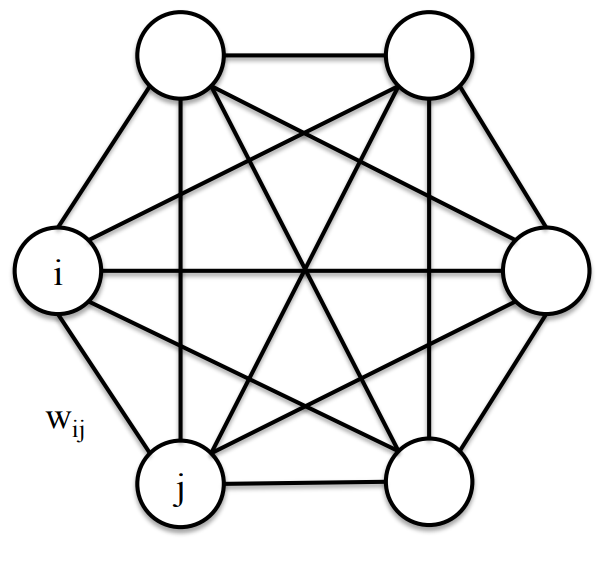
\includegraphics[width=0.3\linewidth]{graphics/Hopfield_Netzwerk.png}
    \caption{Figure of a hopfield network}
\end{figure}
The exemplary network has 6 neurons and bidirectional weigths \( W_{ij} \) between the neurons. 
In addition to that, a Hopfield network has no input or output layer.\footcite[Vgl.][3]{yaoMassivelyParallelAssociative2013}
The main goal is to find the values for each neuron in the network given a specific input that minimizes the total energy of the system.\footcite[Vgl.][7]{ahadNeuralNetworksWireless2016}
The minimum energy is then equal to the state where the network is able to perform as a memory item.\footcite[Vgl.][7]{ahadNeuralNetworksWireless2016}
This energy state can be calculated with the following energy equation\footcite[Vgl.][2556]{hopfieldNeuralNetworksPhysical1982}: 

\begin{equation}
    E = -\frac{1}{2} \sum_{i \neq j} T_{ij} V_i V_j .
\end{equation}
This energy function invented by Hopfield has big similarities with a \ac{BM} when comparing to the
equation 2.4. This is one of the reasons why the execution on the Memristor Hopfield Network could work out.
When comparing a Hopfield Network, they seek to achieve the effect of changing node activation on the overall energy of the network but \ac{BM}s replace this with the probability of a certain node being activated on the network energy.\footcite[Vgl.][7]{ahadNeuralNetworksWireless2016}
The second important reason to research the hopfield networks is for their updating process.
Approximately, the acitivity rule for each neuron is to update its state as if it were a single neuron with the threshold activation function.\footcite[Vgl.][506]{mackayInformationTheoryInference2003}
\[
s_i \leftarrow 
\begin{cases} 
+1 & \text{if } \sum_j w_{ij} s_j + b \geq \theta_i, \\
-1 & \text{otherwise}.
\end{cases}
\]

The state of the neuron will be updated to 1 if the sum over all weights multiplied with the states \{1, -1\} added to a bias \( b \)  is greater than the threshold \( \theta_i \).
In the case of our accelerator the threshold is set to 0 but in theory can be used as an hyperparameter.

Since every neuron's output is an input to all the other neurons the order of the updates need to be specified.\footcite[Vgl.][506]{mackayInformationTheoryInference2003}
There is the possbility to update all neurons synchronous or asynchronous. 
There is no study that shows what update method leads to better results.
Therefore, this paper follows the asynchronous option and ensures to do enough iterations, so that every neuron has at least updated once before moving on.
In addition to that, the idea of the updating method of the accelerator is slightly different. The idea behind this is to inject noise into the system so that the acitivation function could work together with the activation function that a \ac{RBM} needs to perform. 
In detail the idea is to add a normal gaussian distribution \( g(x) \) on top of the activation function.\footcite[Vgl.][4-5]{bohmNoiseinjectedAnalogIsing2022}
As a result the new statistical updating function looks like the following:
\[
s_i \leftarrow 
\begin{cases} 
+1 & \text{if } \sum_j w_{ij}  + b + g(x) \geq \theta_i, \\
-1 & \text{otherwise}.
\end{cases}
\]

Now the system could potentially be used to update the states of the neurons within a \ac{RBM}.
Since the success of this method is not guaranteed or tested in literature yet the practical part first needs to validate if this concept is feasible.

\subsection{Crossbar}
\subsection{Output Hopfield Network}
\subsection{Noisy HNN}
